\begin{pastexam}[label={px:gk3-115-ds-02}]{高考三級資訊處理 115 年 第二題}
（申論；25 分）

給定一個無向圖$\mathrm{G} = (\mathrm{V}, \mathrm{E})$，每個頂點代表一個地點，每條邊$e\ (e \in \mathrm{E})$代表一條
道路，邊的正整數權重$\omega(e)$表示該道路的塞車程度，數值越大越壅塞。對於一條從起點 $s$ 到終點
$t\,(s, t \in \mathrm{V})$的路徑 P，其最大塞車程度$\mathrm{C(P)}$定義為路徑上所有邊權重的最大值：
\[
\mathrm{C(P)} = \max_{e \in P} \omega(e)
\]
本題透過修改 Dijkstra 最短路徑演算法中陣列 $d$ 的定義與更新方式，求出從 $s$ 到 $t$ 可行路徑所能達到的「最大
塞車程度的最小值」。修改後的演算法流程與 Dijkstra 最短路徑演算法相同，差異僅在於$d[v]\,(v \in \mathrm{V})$的
定義與更新規則，其中，新的$d[v]$表示目前已知從 $s$ 到 $v$ 的路徑中，最大邊權重的最小值。初始時令$d[s] = 0$，
其他頂點 $v$ 的$d[v] = \infty\,(v \ne s)$。之後依照 Dijkstra 演算法，每一輪選出尚未被選定且 $d$ 值最小的頂點
$u$，並將原本的更新方式$d[v] = \min(d[v], d[u] + \omega(u,v))$改為$d[v] = \min(d[v], \max(d[u], \omega(u,v)))$，
其中$\omega(u,v)$為邊$(u,v)\,(u, v \in \mathrm{V})$的權重。重複進行，直到終點 $t$ 被選定為止。
\begin{itemize}[leftmargin=2.2em]
\item[㈠] 以下列無向圖為例，令起點 $s$ 為 A，終點 $t$ 為 F，依照修改後的演算法，逐步列出每次選定一個頂點後
陣列 $d$ 的變化過程。陣列中的頂點順序請依字母順序排列。（15 分）
\begin{center}
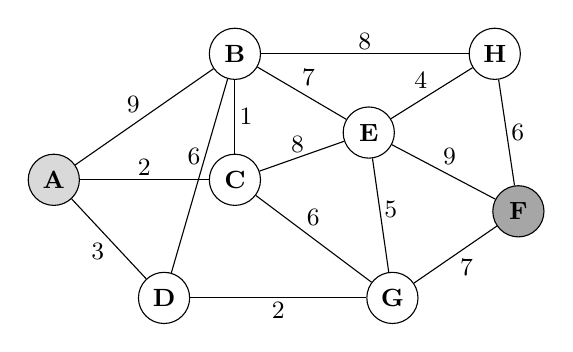
\begin{tikzpicture}[v/.style={circle,draw,minimum size=6.5mm,inner sep=0pt,font=\small\bfseries},
  w/.style={font=\small,inner sep=1.5pt}]
\node[v,fill=black!15] (A) at (0,0) {A};
\node[v] (B) at (2.3,1.6) {B};
\node[v] (C) at (2.3,0) {C};
\node[v] (D) at (1.4,-1.5) {D};
\node[v] (E) at (4.0,0.6) {E};
\node[v,fill=black!35] (F) at (5.9,-0.4) {F};
\node[v] (G) at (4.3,-1.5) {G};
\node[v] (H) at (5.6,1.6) {H};
\draw (A) -- node[w,above left] {9} (B);
\draw (A) -- node[w,above] {2} (C);
\draw (A) -- node[w,below left] {3} (D);
\draw (B) -- node[w,right] {1} (C);
\draw (B) -- node[w,pos=0.4,left] {6} (D);
\draw (B) -- node[w,above] {8} (H);
\draw (B) -- node[w,above right,pos=0.45] {7} (E);
\draw (C) -- node[w,above,pos=0.45] {8} (E);
\draw (C) -- node[w,above right,pos=0.4] {6} (G);
\draw (E) -- node[w,above left] {4} (H);
\draw (E) -- node[w,above right,pos=0.45] {9} (F);
\draw (E) -- node[w,right,pos=0.45] {5} (G);
\draw (H) -- node[w,right] {6} (F);
\draw (G) -- node[w,below right] {7} (F);
\draw (D) -- node[w,below] {2} (G);
\end{tikzpicture}
\end{center}
\item[㈡] 說明修改後演算法之正確性，是基於$d[v]$更新規則具有何種性質。（5 分）
\item[㈢] 假設圖以相鄰串列（adjacency list）表示。若要在尚未選定的頂點中找出 $d$ 值最小者，可使用以下兩種方法：\\
方法一：每次以線性方式掃描所有尚未選定的頂點找出最小 $d$ 值。\\
方法二：使用最小堆積（min-heap）維護目前 $d$ 值最小的頂點。\\
分別就這兩種方法，分析修改後演算法最壞情況的時間複雜度。（5 分）
\end{itemize}
\end{pastexam}

\begin{pastsoln}
答案：㈠ 依序選定 A, C, B, D, G, E, H, F，最後 $d[\mathrm{F}] = 6$（路徑 A--D--G--E--H--F）。 ㈡ 單調性：
$\max(d[u], \omega(u,v)) \ge d[u]$，路徑往後延伸時 $C$ 值不會變小。 ㈢ 方法一 $O(|V|^2)$；方法二
$O((|V| + |E|)\log |V|)$。

\textbf{㈠} 每選定一個頂點 $u$，就對 $u$ 每個尚未選定的鄰居 $v$ 做 $d[v] \gets \min(d[v], \max(d[u], \omega(u,v)))$。
下表每一列是選定該頂點並更新完之後的 $d$（$\infty$ 記為 $\infty$，方框表示已選定，粗體是這一輪改變的值）：
\begin{center}
\small
\setlength{\tabcolsep}{5pt}
\begin{tabular}{lcccccccc}
\toprule
選定 & A & B & C & D & E & F & G & H \\
\midrule
初始 & 0 & $\infty$ & $\infty$ & $\infty$ & $\infty$ & $\infty$ & $\infty$ & $\infty$ \\
A & \fbox{0} & \textbf{9} & \textbf{2} & \textbf{3} & $\infty$ & $\infty$ & $\infty$ & $\infty$ \\
C & \fbox{0} & \textbf{2} & \fbox{2} & 3 & \textbf{8} & $\infty$ & \textbf{6} & $\infty$ \\
B & \fbox{0} & \fbox{2} & \fbox{2} & 3 & \textbf{7} & $\infty$ & 6 & \textbf{8} \\
D & \fbox{0} & \fbox{2} & \fbox{2} & \fbox{3} & 7 & $\infty$ & \textbf{3} & 8 \\
G & \fbox{0} & \fbox{2} & \fbox{2} & \fbox{3} & \textbf{5} & \textbf{7} & \fbox{3} & 8 \\
E & \fbox{0} & \fbox{2} & \fbox{2} & \fbox{3} & \fbox{5} & 7 & \fbox{3} & \textbf{5} \\
H & \fbox{0} & \fbox{2} & \fbox{2} & \fbox{3} & \fbox{5} & \textbf{6} & \fbox{3} & \fbox{5} \\
F & \fbox{0} & \fbox{2} & \fbox{2} & \fbox{3} & \fbox{5} & \fbox{6} & \fbox{3} & \fbox{5} \\
\bottomrule
\end{tabular}
\end{center}
各輪的計算：
\begin{itemize}
\item 選 A（$d = 0$）：B $= \max(0, 9) = 9$，C $= \max(0, 2) = 2$，D $= \max(0, 3) = 3$。
\item 選 C（$d = 2$，最小）：B $= \min(9, \max(2, 1)) = 2$；E $= \max(2, 8) = 8$；G $= \max(2, 6) = 6$。
\item 選 B（$d = 2$）：D $= \min(3, \max(2, 6)) = 3$ 不變；E $= \min(8, \max(2, 7)) = 7$；H $= \max(2, 8) = 8$。
\item 選 D（$d = 3$）：G $= \min(6, \max(3, 2)) = 3$。
\item 選 G（$d = 3$）：E $= \min(7, \max(3, 5)) = 5$；F $= \max(3, 7) = 7$。
\item 選 E（$d = 5$）：F $= \min(7, \max(5, 9)) = 7$ 不變；H $= \min(8, \max(5, 4)) = 5$。
\item 選 H（$d = 5$）：F $= \min(7, \max(5, 6)) = 6$。
\item 選 F（$d = 6$）：終點被選定，停止。
\end{itemize}
所以從 A 到 F 的「最大塞車程度的最小值」是 $6$。 往回追每個 $d$ 值最後是被誰更新的：F 來自 H，H 來自 E，E 來自
G，G 來自 D，D 來自 A，路徑是 A--D--G--E--H--F，邊權 $3, 2, 5, 4, 6$，最大值 $6$。 （其他路徑例如 A--C--G--F
的最大值是 $7$，A--D--G--F 也是 $7$。）

\textbf{㈡} 正確性靠的是更新規則的\textbf{單調性}（不遞減）：路徑往後多接一條邊 $(u, v)$，新的瓶頸值
$\max(d[u], \omega(u, v)) \ge d[u]$，絕不會比原來的小。 這和原本 Dijkstra 要求「邊權非負」是同一個角色：
$d[u] + \omega \ge d[u]$（資結書第~25.2~節）。 有了它，Dijkstra 的論證照樣成立：當 $u$ 是未選定頂點中 $d$ 最小
的，任何一條從 $s$ 到 $u$ 的路徑，在離開已選定集合的那一點之後，瓶頸值已經 $\ge$ 那個未選定頂點的 $d$，
$\ge d[u]$，之後只會變大不會變小，所以不可能比 $d[u]$ 更好，$d[u]$ 在選定時已經是最佳值。 另外 $\max$ 也滿足
「最佳子結構」：$s$ 到 $v$ 的最佳路徑，前段可以換成 $s$ 到 $u$ 的最佳路徑而不變差，因為 $\max(\cdot, \omega)$
是單調函數。

\textbf{㈢} 設 $n = |V|$、$m = |E|$。 演算法共選 $n$ 輪（最壞情況 $t$ 最後才選到），每條邊最多被鬆弛兩次（無向
圖兩端各一次），每次更新 $O(1)$。
\begin{itemize}
\item \textbf{方法一}：每輪線性掃描未選定的頂點 $O(n)$，共 $n$ 輪 $O(n^2)$；更新鄰居總共 $O(m)$。 合計
$O(n^2 + m) = O(n^2) = O(|V|^2)$（簡單圖 $m < n^2$）。
\item \textbf{方法二}：堆積裡最多 $n$ 個頂點。 取出最小值 $n$ 次，每次 $O(\log n)$；每次 $d[v]$ 變小就做一次
decrease-key（或再插入一筆），最多 $O(m)$ 次，每次 $O(\log n)$。 合計 $O((n + m)\log n) = O(|E| \log |V|)$
（連通圖 $m \ge n - 1$）。
\end{itemize}
稠密圖（$m = \Theta(n^2)$）時方法一的 $O(n^2)$ 較好；稀疏圖（$m = O(n)$）時方法二的 $O(n \log n)$ 較好。
\end{pastsoln}
